%qqqqqqqqqqqqqqqqqqqqqqqqqqqqqqqqqqqqqqqqqqqqqqqqqqqqqqqqqqqqqqqqqqqqqqqqq
%Quote
\begin{savequote}[50mm]
‘‘The most incomprehensible thing about the universe is that it is 
comprehensible’’
\qauthor{Albert Einstein}
\end{savequote}
%qqqqqqqqqqqqqqqqqqqqqqqqqqqqqqqqqqqqqqqqqqqqqqqqqqqqqqqqqqqqqqqqqqqqqqqqq




%#########################################################################
\chapter{The Cosmological Environment and the Local Group}
\label{cha:Results}


%Reviewed
In this chapter, it is presented the results obtained from the simulations 
des\-cribed in the previous chapter \ref{cha:N-BodySimulations} for the 
dependence of the properties of LG-like systems on the cosmological 
environment in which they are embedded. It is firstly characterized each 
one of the used simulations (CLUES and Bolshoi) with the aim to guarantee 
consistency between the used cosmologies and between the distribution of 
the environmental properties (see section 
\ref{sec:StatisticalPropertiesOfAllSimulations}). After this, in the 
section \ref{sec:PropertiesOfSamplePairs} it is determined the physical
and statistical properties of each one of the defined samples in
\ref{subsec:SampleOfPairsToUse} and it is analysed the correlations 
between the computed properties and the cosmological environment of each 
simulation.



%#########################################################################




%*************************************************************************
%Statistical properties of all simulations
\section{Properties of the Simulations}
\label{sec:StatisticalPropertiesOfAllSimulations}


%Reviewed
One of the first steps for determining the influence of the 
environment on LG-like systems is to construct a \textit{CLG} sample in
unconstrained simulations and thereby obtaining a more robust statistics.
In order to guarantee the consistency of this sample is necessary to 
stablish the equivalence between the distributions of dark matter halos
and analyse the distributions of the cosmological environment of each 
simulation.



	%---------------------------------------------------------------------
	%Halos Properties
	\subsection{Halo Mass Function}
	\label{subsec:Halos_Properties}
	%---------------------------------------------------------------------


%Reviewed
The spatial distribution of the halos exhibits the fine structure of the 
cosmic web, which it is constituted by dark matter. This is exhibited both 
in simulations (see Figure \ref{fig:Halos_Web}) and in cosmological 
observations (see section \ref{sec:CosmologicalObservations}). This 
suggests possible correlations between the properties of the halos and the
environment in which they are embedded, such as it has been demonstrated 
for dark matter halo shapes, the spin parameter and the alignment of 
satellite halos in \cite{libeskind2013}, and for the halo mass 
\cite{lemson1999}. Specially, in the work of \cite{libeskind2013} it is
demonstrated that the V-web classification scheme is more appropriated for
studying correlations with respect to directional properties, like the 
angular momentum of \textit{IP} or \textit{CLG} systems in the section 
\ref{sec:PropertiesOfSamplePairs}.


%Reviewed
\
%.........................................................................
%FOF method in CLUES simulation
\begin{figure}[htbp]
	\centering
	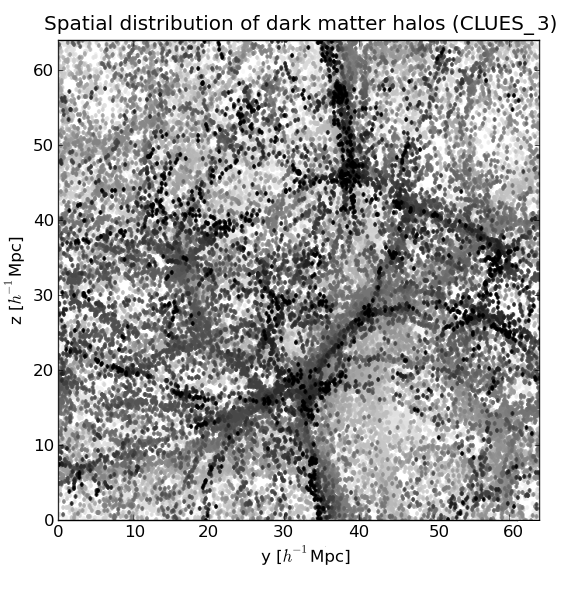
\includegraphics[width=0.58\textwidth]
	{./figures/3_nbody_simulations/Halos_Spatial_Distribution(CLUES_16953).png}

	\caption{\small{Spatial distribution of dark matter halos, exhibiting
	the	characteristic structure of the cosmic web. The colour gradient 
	indicates the depth with respect to the $x$ axis, where black dots 
	are the nearest halos.}}
	
	\label{fig:Halos_Web}
\end{figure}
%.........................................................................


%Reviewed
According to the defining conditions of the \textit{IP} and \textit{CLG} 
samples presented in the subsection \ref{subsec:SampleOfPairsToUse}, the
main property of the halos that is necessary for cons\-tructing these samples
is the halo mass. Therefore it is important to stablish the equivalence 
between the mass distribution of each simulation. The next Figure 
\ref{fig:IMF} shows the results of calculating the cumulative mass 
functions for the Bolshoi simulation and for the three CLUES simulations.


%Reviewed
%.........................................................................
%Integrated Mass Fraction
\begin{figure}[htbp]
	\centering
	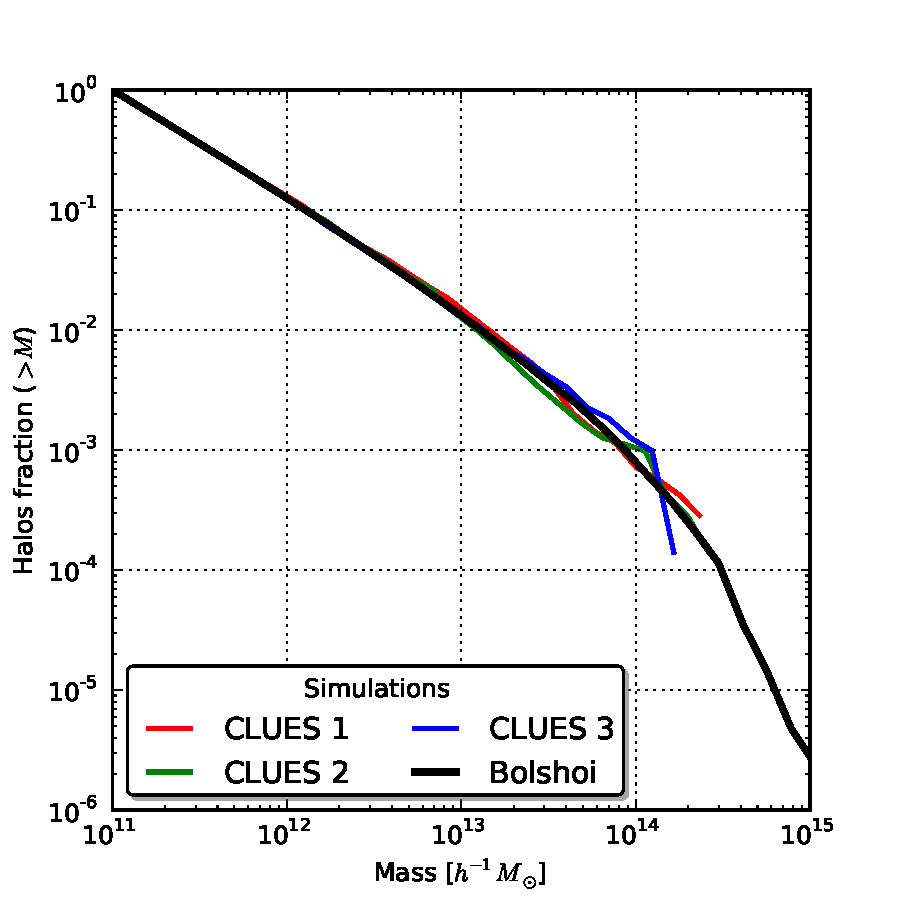
\includegraphics[width=0.70\textwidth]
	{./figures/4_results/Halos_IMF.pdf}
	
	\caption{\small{Cumulative mass functions of the dark matter halos
	(\textit{GH} sample) for each simulation.}}
	\label{fig:IMF}
\end{figure}
%.........................................................................


%Reviewed
For high mass values, the distributions are slightly different due to the 
smaller number of halos in the CLUES simulations, what makes the statistics
less significant in this case. In spite of this, within the mass range 
where the \textit{IH} samples are defined ($5.0 \times 10^{11}\Msun - 
5.0\times 10 ^{12}\Msun$), the distributions are consistent with the 
Press-Schechter mass function formalism \cite{press1974} using the 
cosmological parameters of WMAP7, thereby indicating the equivalence 
between the defined samples for all the used simulations.




	%---------------------------------------------------------------------
	%Environment Properties
	\subsection{Distributions of the Cosmological Environment}
	\label{subsec:Environment_Properties}
	%---------------------------------------------------------------------



%Reviewed
As it has been shown in the section \ref{sec:EnvironmentCharacterization},
the characterization of the cosmological environment is reached by using
physical quantities that indicate the geometric or the dynamical local 
nature of a certain region in the spatial matter distribution. Specially, 
the V-web scheme allows to give account of the dynamics at smaller scales 
of the cosmic web, thereby allowing to characterize and define an adequate 
host environment for halos and other cosmological structures. The next 
Figure shows the results of calculating the distributions for each one of
the eigenvalues of the shear velocity tensor (distributions of 
environment), for both, the cells of the simulations, and the host cells
of the halos of the \textit{GH} sample.


%Reviewed
%.........................................................................
%1D Distribution of Vweb eigenvalues in cells
\begin{figure}[htbp]
	\centering
	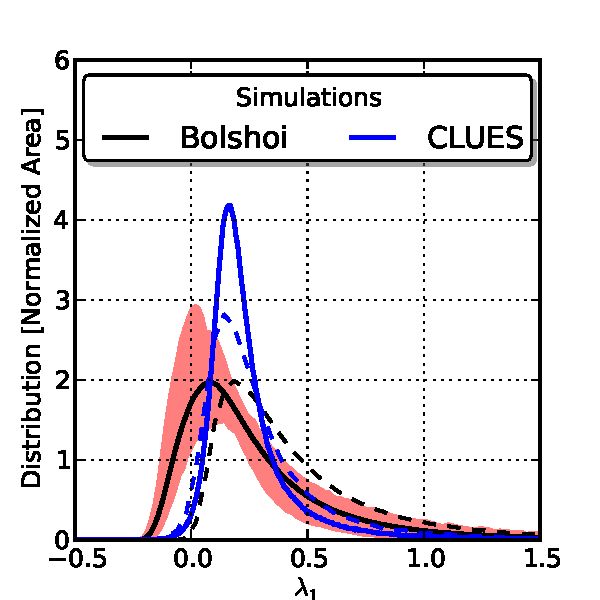
\includegraphics[width=0.38\textwidth]
	{./figures/4_results/Cells_Distro_L1.pdf}
	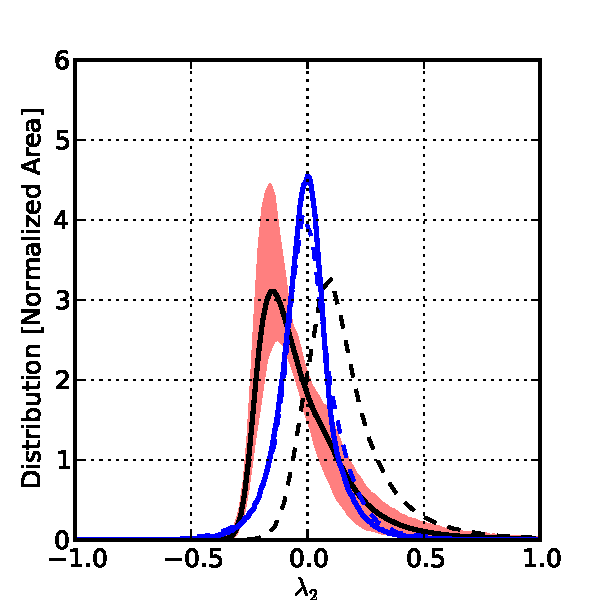
\includegraphics[width=0.38\textwidth]
	{./figures/4_results/Cells_Distro_L2.pdf}
	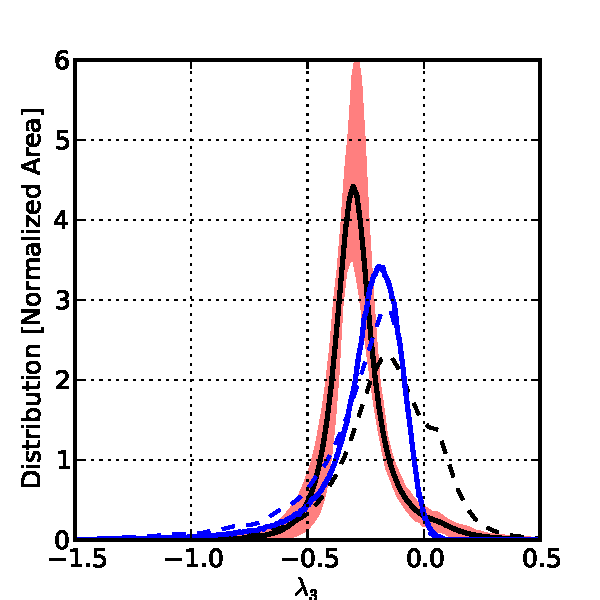
\includegraphics[width=0.38\textwidth]
	{./figures/4_results/Cells_Distro_L3.pdf}

	\caption{\small{ Distributions of eigenvalues of the V-web scheme 
	calculated over all the volume cells (continuous lines) and over the 
	host cells of the dark matter halos defined in the FOF catalogue (dashed 
	lines). All the distributions are normalized such that their area is
	the unity. Resolution of $1.0 h^{-1}$ Mpc/cell and softening parameter
	of one cell size.}}
	\label{fig:1D_Cells_Eigenvalues}
\end{figure}
%.........................................................................


%Reviewed
The main result of the Figure \ref{fig:1D_Cells_Eigenvalues} consists in 
the difference of the distributions for all the volume cells (continuous 
lines) between the Bolshoi simulation and the CLUES simulations \footnote{ 
Because of the high similitude between the distributions of the three 
CLUES simulations, and with the aim of obtaining a more significant 
statistics, they have been merged.}. The effect of the cosmic variance 
(red regions) is included from the calculation of the distributions of 
environment over $64$ sub-volumes of the Bolshoi simulation, with a 
similar size than the CLUES simulations. In spite of this, the 
distributions of environment of the CLUES simulations are outside the 
region of cosmic variance, thereby indicating a different cosmological 
large-scale structure between both simulations.


%Reviewed
A second important result shown by the Figure 
\ref{fig:1D_Cells_Eigenvalues} it is obtained from the distributions of
environment for halos (continuous lines). In the case of Bolshoi, it is
noticed an important bias between the distribution of environment 
associated to the volume cells and the host cells of the halos, thereby 
indicating that the spatial distribution of the halos is not a good tracer
of the large-scale structure of the matter field. This result is 
consistent with the work of \cite{libeskind2013}, where it has been found
an important bias in the distributions of environment according to 
different mass ranges of the halos, also using the Bolshoi simulation. In
the case of the CLUES simulations, the distributions of environment of the
halos are significantly less bia\-sed regarding the volume cells, thus 
indicating for this case that halos do distribute spatially according to
the cosmological environment quantified by using the V-web scheme.


%Reviewed
Finally, in the Figure \ref{fig:Vol_Fraction} it is shown the calculated
mean densities and the vo\-lume fractions for each type of region (see 
section \ref{sec:EnvironmentCharacterization}) according to the threshold
value $\lambda_{th}$. The volume fraction functions are different between
the CLUES and Bolshoi simulations, specially for values close to 
$\lambda_{th} = 0.1$, corresponding to sheet regions. This is due to the 
relative displacement of the peaks of the distributions of environment for
each simulation (see Figure \ref{fig:1D_Cells_Eigenvalues}), what implies
a different behaviour before the criterion to classify the type of region 
from the $\lambda_{th}$ value. In spite of this, the volume fractions are
more or less consistent for both simulations within the range $0.2 \leq 
\lambda_{th} \leq 0.4$ that corresponds to the range where the visual 
impression of the overall density field is better reproduced.


%Reviewed
\newpage
%.........................................................................
%Volume Fraction
\begin{figure}[htbp]
	\centering
	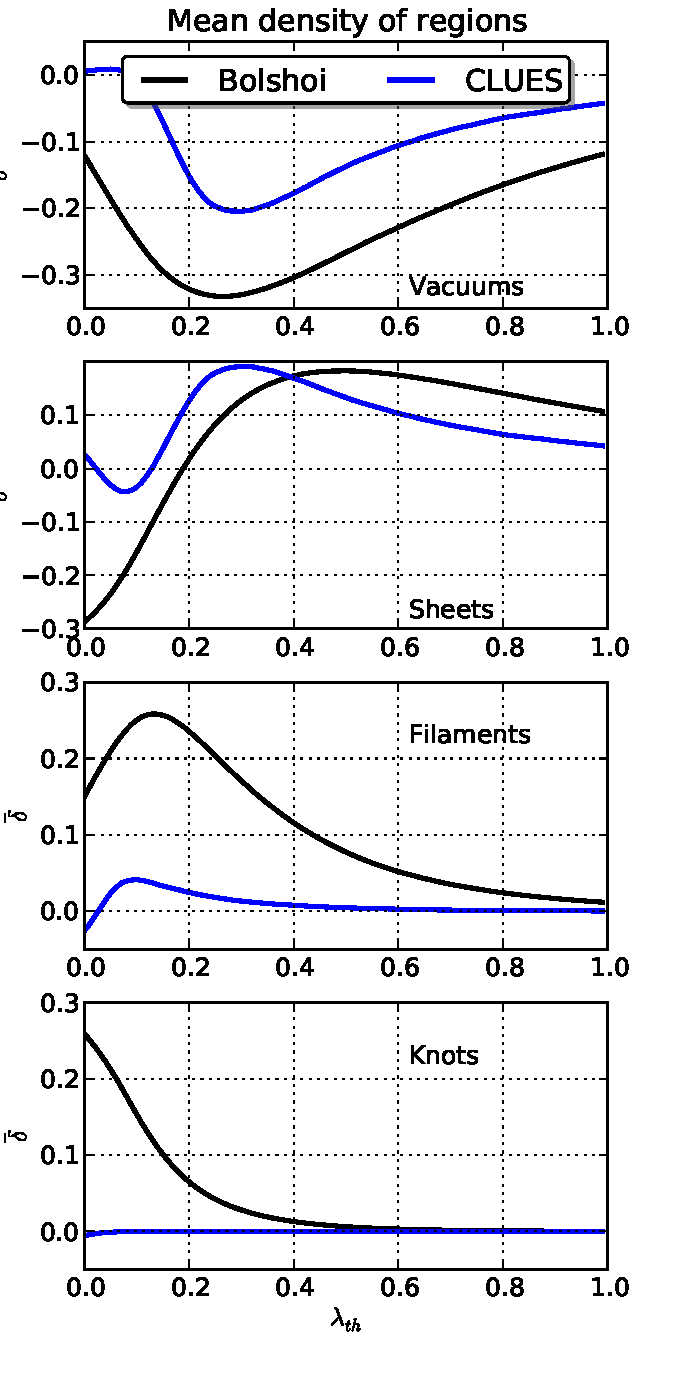
\includegraphics[width=0.43\textwidth]
	{./figures/4_results/Density_Regions.pdf}
	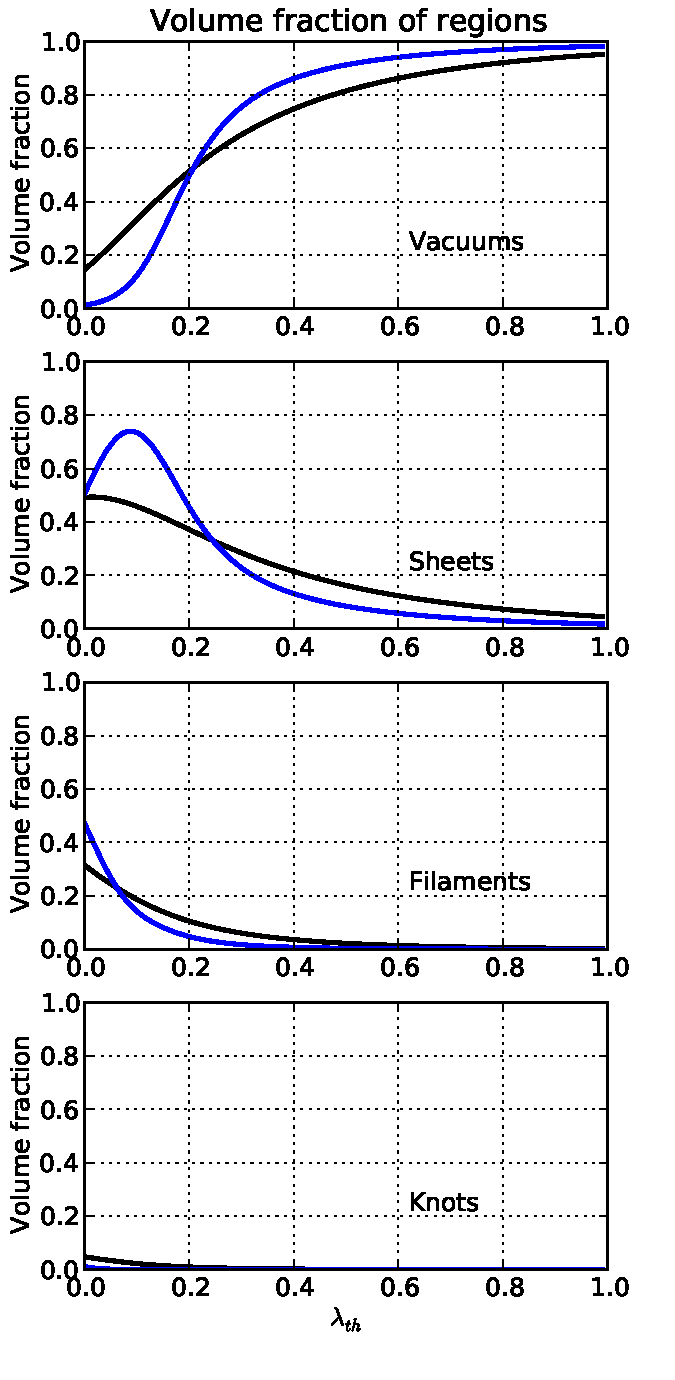
\includegraphics[width=0.43\textwidth]
	{./figures/4_results/Volume_Regions.pdf}
	
	\caption{\small{Mean density parameter for different type of 
	regions in terms of the thre\-shold value $\lambda_{th}$ (left panels).
	Volume fractions normalized for different type of regions, also 
	according to the threshold value $\lambda_{th}$ (right panels).}}
	\label{fig:Vol_Fraction}
\end{figure}
%.........................................................................


%Reviewed
In the figures of the mean density for each type of region, it is shown 
important results regarding the cosmological environment. The first thing
that can be noticed is the difference between the mean densities of both 
simulations for each type of region. For instance for vacuum regions, in
Bolshoi these correspond to regions with a mean density much less than 
the mean density of the entire simulation, whereas in the CLUES 
simulations, the sub-density of vacuum regions is not very pronounced.
Due to the small fraction of knot regions in both simulations (because 
their zero-dimensional geometry), the global structure of the cosmic web
can be understood just in terms of the spatial distribution of vacuums,
sheets and filaments, being filaments the counterpart of vacuums regarding
the density parameter. From this it is expected that the difference 
of the sub-density values of vacuum regions between both simulations 
becomes compensated with a pronounced difference of the over-density 
values of filament regions between both simulations too. The latter has been 
obtained in the same figure, where it can be seen that filament regions of
the Bolshoi simulation are notably denser than filaments in CLUES. In the
case of sheet regions, these correspond to regions with intermediate 
values of density, within a range between filaments and vacuums, therefore
it is expected that the difference of the mean density of these 
regions between both simulation is not very pronounced, such as it can be 
noticed in the same figure.


%Reviewed
%.........................................................................
%Vweb Comparison
\begin{figure}[htbp]
	\begin{center}
	\makebox[\textwidth]{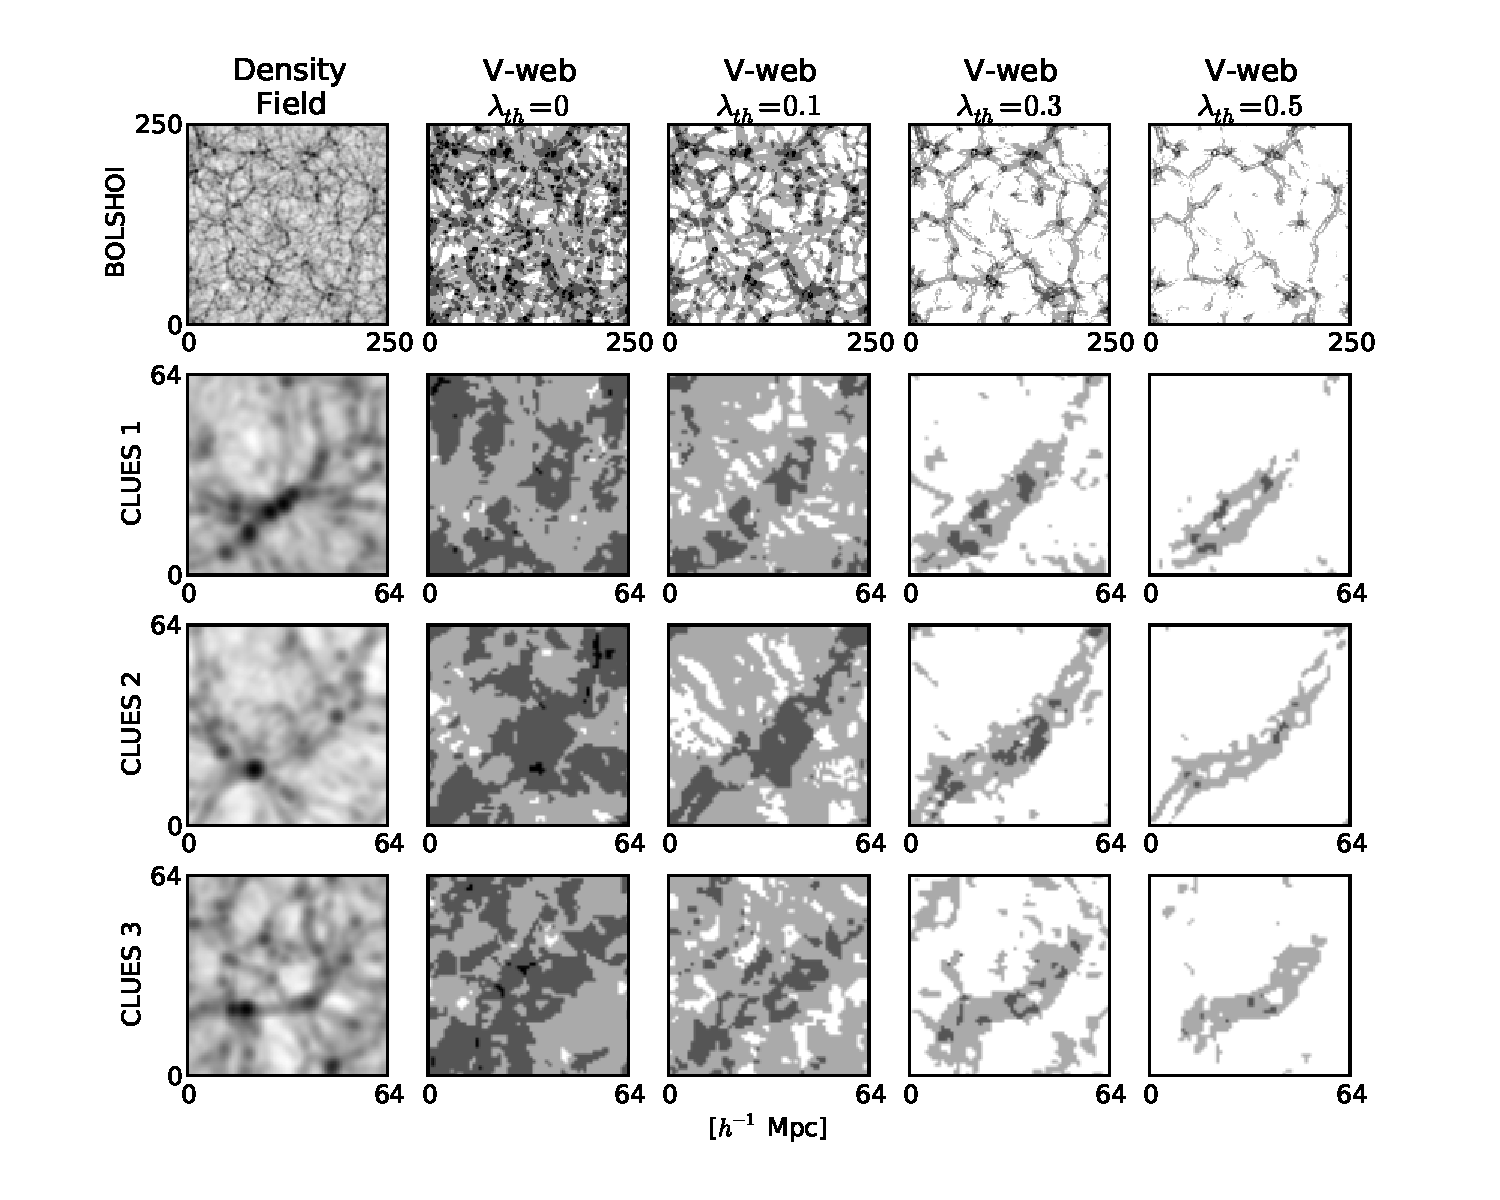
\includegraphics[trim = 10mm 10mm 10mm 9mm, clip,
	width=0.63\paperwidth,angle=0]
	{./figures/4_results/Vweb_Comparison.pdf}}
	\end{center}	
	
	\caption{\small{Comparison between the visual impression obtained by 
	the	V-web scheme for several values of the threshold parameter 
	$\lambda_{th}$. It is used the next classification scheme (Black - Knot,
	Dark gray - Filament, Gray - Sheet, White - Vacuum). The resolution of
	each grid is $1.0 h^{-1}$ Mpc/cell with a Gaussian softening of one cell
	size. The width of each slide is one cell.}}
	\label{fig:Vweb_Comparison}
\end{figure}
%.........................................................................


%Reviewed
The second result shown in the Figure \ref{fig:Vol_Fraction} consists in
determining an optimal threshold parameter $\lambda_{th}$ for reproducing
the visual impression of the cosmic web. As it is shown in this figure,
the volume fractions associated to vacuums and sheets are relatively high
regarding the values of filaments and knots, and this for all the swept 
range of threshold values $\lambda_{th}$. From this it is expected that 
the visual impression of the large-scale matter field is completely 
dominated by the spatial distribution of vacuums and slightly less by 
filaments and sheets. In the case of a low value of the $\lambda_{th}$ 
parameter, e.g. $\lambda_{th}<0.2$, the mean density parameter of sheet 
regions becomes negative, thereby indicating that possibly these regions 
are invading zones that should be catalogued as vacuums, such as it can be 
noticed in the Figure \ref{fig:Vweb_Comparison} for $\lambda_{th} = 0$ o 
$\lambda_{th} = 0.1$. In the case of high values, e.g. $\lambda_{th} > 
0.4\sim 0.5$, the mean density parameter for vacuums is increasing, thus 
indicating that these regions are invading high density zones, which at 
first should be sheets or filaments. This can be noticed in the Figure 
\ref{fig:Vweb_Comparison} for $\lambda_{th} = 0.5$, where all the volume 
is widely dominated by vacuums, thereby loosing the characteristic 
structure of the cosmic web. This analysis suggests that the optimal value
of $\lambda_{th}$ may be that where the mean density of vacuum regions is 
minimized , since this type of region is the most dominant. A result that 
supports this hypothesis is that the found value of $\lambda_{th}$ for 
both simulations is quite similar $\lambda_{th}\approx 0.3$, and 
coincides with the value obtained qualitatively by fitting at first glance 
the visual impression of the cosmological environment.


%Reviewed
To conclude this section, it is discussed the results obtained for the 
distributions of environment. In spite of there is a significant bias 
between the spatial distribution of dark matter halos and the distribution
of the matter field in the Bolshoi simulation, contrary case in the CLUES 
simulations, and there is a marked difference between the mean densities
associated to each type of region for both simulations, the objective of 
constructing a \textit{CLG} sample in the Bolshoi simulation from the 
\textit{LG} systems found in CLUES, as it was mentioned in the chapter 
\ref{cha:N-BodySimulations}, it is to obtain a more faithful sample of 
isolated pairs that also reproduces the same local environment of those
\textit{LG} systems. Then, it is expected that the local dynamic, 
quantifying by the V-web scheme, is independent of the difference between
the distributions mentioned above, retaining the validity of the proposed
construction scheme for the \textit{CLG} sample.



%*************************************************************************




%*************************************************************************
%Properties of sample pairs
\section{Properties of the \textit{CLG} Sample}
\label{sec:PropertiesOfSamplePairs}


%Reviewed
Once it has been determined the consistency between the defined samples 
for both simulations, the next step is to determine their properties. It 
is of special interest to analyse the \textit{CLG} sample in Bolshoi, 
taking as the control sample the \textit{IP} sample, and as the reference 
sample the \textit{LG} sample in CLUES.



	%---------------------------------------------------------------------
	%Determination of their host environment
	\subsection{Determining the Environment}
	\label{subsec:DeterminationOfTheirHostEnvironment}
	%---------------------------------------------------------------------


%Reviewed
As it has been defined in the subsection \ref{subsec:SampleOfPairsToUse} of
the last chapter, the \textit{CLG} sample in the Bolshoi simulation is 
constructed by imposing on the \textit{IP} sample the extra condition of 
reproducing the cosmological environment of the LG-like systems found into 
the CLUES simulations. The main aim of doing this, it is to find a sample 
in the Bolshoi simulation analogous to the \textit{LG} sample, regarding 
their physical properties as well as their abundance. With respect to the 
latter, it is natural to assume, considering the consistency between the 
simulation already determined, that the abundance of a certain sample 
should scale approximately as the volume of the simulation. This fact can
be considered as the first success of the proposed construction scheme, 
since it is reproduced approximately this scale law for the \textit{CLG} 
sample in Bolshoi and the \textit{LG} samples in CLUES (see Table 
\ref{tab:Samples}).


%Reviewed
In spite of the latter, this construction scheme just consists of a cut
in the \textit{IP} sample with respect to the eigenvalues of the shear
velocity tensor of the V-web, evaluated over the host cells of the pair 
systems, which does not imply an adequate reproduction of neither the 
physical properties nor the local cosmological environment of LG-like
systems. For this reason, below it will be analysed possible bias in the 
distributions of environment for the host cells of the \textit{CLG} 
systems.


%Reviewed	
%.........................................................................
%Pathogenic Situation
\begin{figure}[htbp]
	\centering
	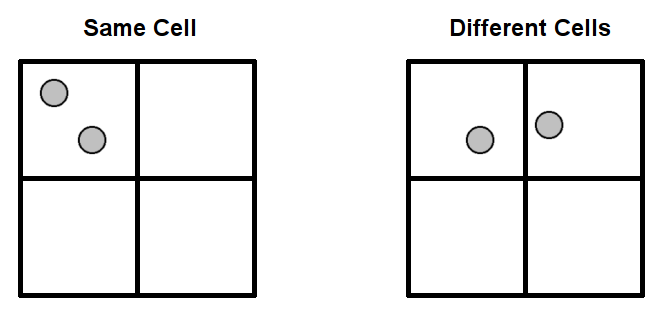
\includegraphics[width=0.5\textwidth]
	{./figures/4_results/Pathogenic_Situation.png}
	
	\caption{\small{Pathological situation regarding the environment of a
	pair system.}}
	\label{fig:Pathogenic_Situation}
\end{figure}
%.........................................................................


%Reviewed
One of the first considerations that should be taken into account for 
quantifying the environment of pair systems (\textit{P}, \textit{IP}, 
\textit{CLG} and \textit{LG} samples), it is that the two halos of the 
pair may be embedded into different cells, such as it is shown in the 
Figure \ref{fig:Pathogenic_Situation}. This pathological situation is 
presented due to the non-point nature of this type of systems and the 
finite resolution of the grid.


%Reviewed
\
%.........................................................................
%Comparison of Lambda in each Halos of Pairs systems
\begin{figure}[htbp]
	\centering
	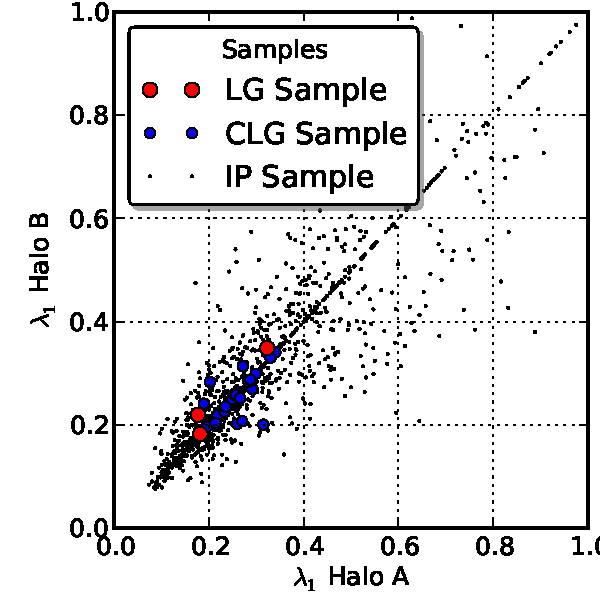
\includegraphics[width=0.46\textwidth]
	{./figures/4_results/CLG_L11_L12.pdf}
	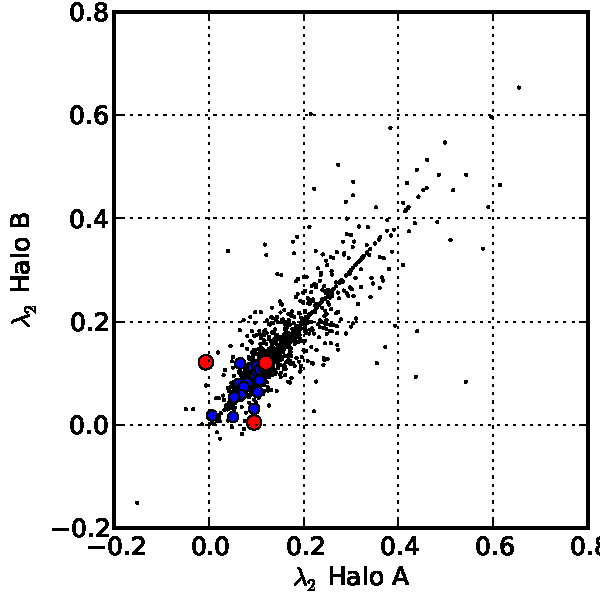
\includegraphics[width=0.46\textwidth]
	{./figures/4_results/CLG_L21_L22.pdf}
	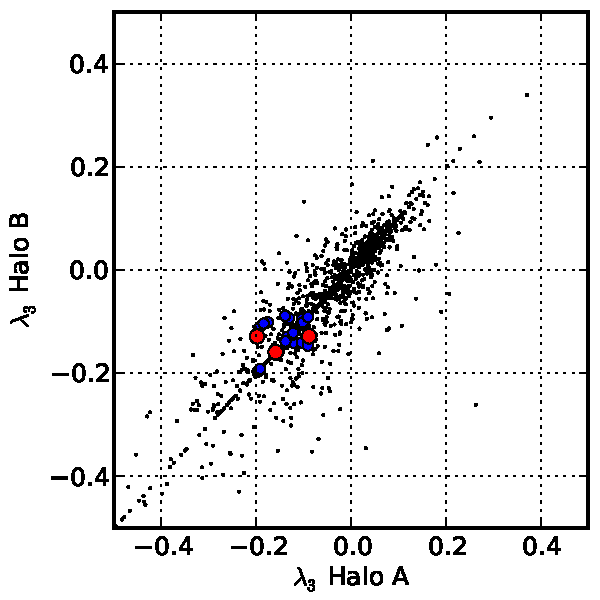
\includegraphics[width=0.46\textwidth]
	{./figures/4_results/CLG_L31_L32.pdf}

	\caption{\small{Comparison between the distributions of the 
	eigenvalues	of the V-web for the two halos of each pair system of
	the \textit{LG}, \textit{CLG} and \textit{IP} samples.}}
	\label{fig:Lambda_Comparison_Pairs}
\end{figure}
%.........................................................................


%Reviewed
In order to quantify this effect, in the Figure 
\ref{fig:Lambda_Comparison_Pairs} are plotted the distributions of each 
eigenvalue of the V-web for each one of the halos in the pair samples. The
ideal situation, where both halos share the same cell, it would correspond
to a straight line with a slope of $45^o$, whereas the pathological 
situations are responsible of the observed dispersion. A way to solve this 
issue is to decrease the resolution of the grid, such that both halos are 
embedded in the same cell, but this would cause a losing of information 
regarding the local environment of the pair system. Due to the Gaussian 
softening of one cell size ($\sim 1 h^{-1}$ Mpc) that has been applied a 
priori over the eigenvalues fields, possible variations between neighbour
cells are neglected, such as it is shown for the most of \textit{IP} 
systems in the figure. Taking into account the latter and the local 
dynamic of pair systems is dominated by the more massive dark halo, by 
convention it will be taken the host cell of this halo as the 
representative of the entire system.


%Reviewed
\
%.........................................................................
%2D Distribution of Vweb eigenvalues in sairs samples
\begin{figure}[htbp]
	\centering
	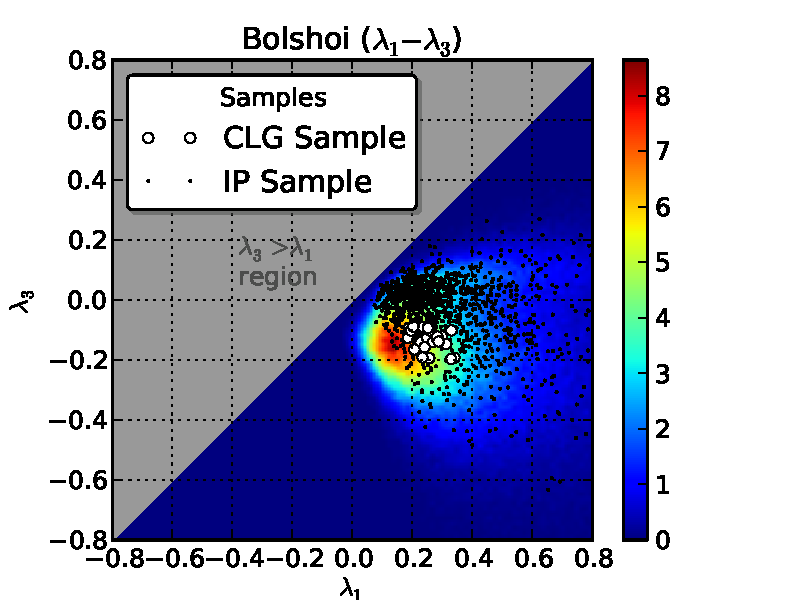
\includegraphics[trim = 0mm 0mm 15mm 0mm, clip, width=0.49\textwidth]
	{./figures/4_results/CLG_Environmet_L1L3.pdf}
	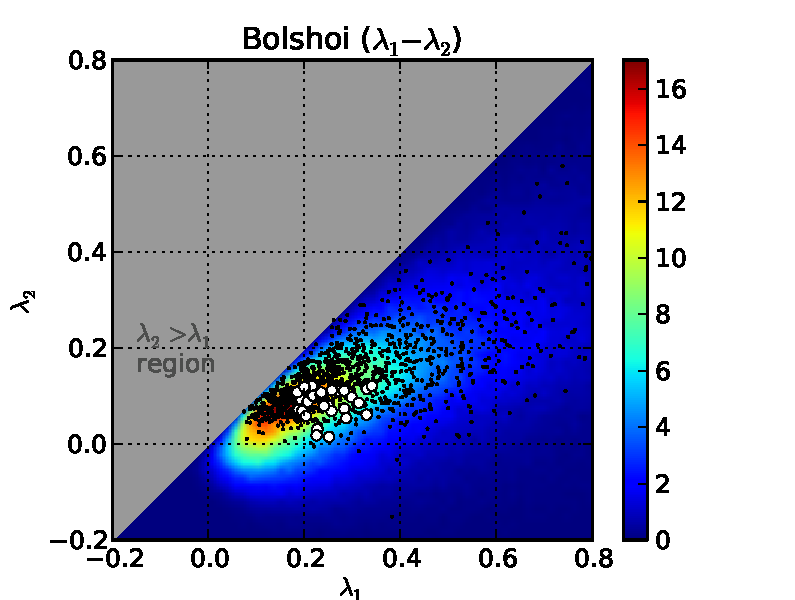
\includegraphics[trim = 0mm 0mm 15mm 0mm, clip, width=0.49\textwidth]
	{./figures/4_results/CLG_Environmet_L1L2.pdf}
	
	\caption{\small{2D distributions of the cosmological environment for
	the defined samples, $\lambda_1$--$\lambda_3$ (left panel) and 
	$\lambda_1$--$\lambda_2$ (right panel). The background histogram, 
	plotted in colours, corresponds to the distribution of environment
	for all the halos in Bolshoi (\textit{GH} sample), its resolution is
	$100\times 100$ for the shown range and it is normalized with respect 
	to its area. The black dots corresponds to the distribution of the 
	\textit{IP} sample and finally the white dots to the \textit{CLG}
	sample.}}
	\label{fig:2D_Samples_Eigenvalues}
\end{figure}
%.........................................................................


%Reviewed
Once it has been determined how to quantify the environment of pair 
systems, in the Figure \ref{fig:2D_Samples_Eigenvalues} is illustrated the
distribution of the samples \textit{GH}, \textit{IP}, \textit{CLG}. As it
has been shown in the subsection \ref{subsec:Environment_Properties}, the
distribution of environment for halos in Bolshoi are considerably biased
with respect to the distribution of the volume cells. In spite of this,
and taking into account that the construction of pair systems it is made
from the sample of halos, it is more interesting to perform comparisons
between the distributions associated to halos (coloured histograms in
the same figure). As it was defined in the subsection 
\ref{subsec:SampleOfPairsToUse}, the \textit{IP} sample is constructed 
such that it is guaranteed its gravitational isolation with respect to
more massive halos and other structures, that is why there are two effects
that compete regarding the distribution of environment of these systems.
In the first effect, it is expected that the abundance of pairs is more
favourable around environments where there are more halos, whereas in the 
second effect, precisely the over-abundance of halos becomes unfavourable
due to the criterion of gravitational isolation. According to the results, 
the second effect is more dominant on the \textit{IP} sample with respect
to all the halos, while for the \textit{P} sample the bias is not longer
presented\footnote{ The latter is not shown in the Figure 
\ref{fig:2D_Samples_Eigenvalues}, but it is easily computed.}
 

%Reviewed
In order to conclude the analysis of the previous figure, it is discussed 
about the distribution of environment for the \textit{CLG} systems in the
Bolshoi simulation. In spite of this distribution is artificially biased 
because of the selection criterion, it is interesting to notice that the
range of the eigenvalues that delimits this sample is relatively reduced, 
thereby indicating that the three LG-like systems in the CLUES simulations
share a similar local dynamic. Although the latter may be an effect 
established a priori by construction due to the constrained nature of the
CLUES simulations, it is still interesting the bias that this feature 
produces on the distribution of environment of the \textit{CLG} sample
regarding all the halos and the \textit{IP} sample.


%Reviewed
To quantify the produced biases in each sample regarding a specific type
of environment (See Figure \ref{fig:ClassificationSchemeTweb}), in the 
next Figure \ref{fig:Samples_Fraction} it is plotted the fractions of 
objects into each type of region. In the optimal range of the threshold 
value $0.2\leq \lambda_{th}\leq 0.4$, defined in the subsection 
\ref{subsec:Environment_Properties}, it is noticed important differences
between each one of the samples, specially for the \textit{CLG}. As it has
been previously mentioned, the effect of the gravitational isolation 
produces a bias between the distribution of environment of the halos 
\textit{GH} and the distribution of the \textit{IP} systems. This can be 
clearly noticed for each one of the number fractions in the optimal range 
of $\lambda_{th}$. In the case of vacuums, the dominant fraction is that 
associated to \textit{IP}, but in the case of sheet regions, the fraction
of both samples are comparable, and even more, in the filament and knot 
regions, the dominant fractions is that corresponding to halos \textit{GH}.
This indicates that \textit{IP} systems are more abundant in regions of 
low to middle density of halos, but even so, there are still a 
considerable fraction within sheet and filament regions, so it is not 
possible to associate a specific type of region to these systems. Finally,
the \textit{CLG} systems present an important bias compared with the two
previously discussed samples, being specially interesting that produces
regarding the \textit{IP} sample, due to the \textit{CLG} sample is a 
sub-sample of this. Again, taking into account the optimal range of
$\lambda_{th}$, it is possible, in this case, to associate a certain type
of region to the \textit{CLG} sample, being these systems preferentially
in sheet and vacuum regions.


%Reviewed
\
%.........................................................................
%Number Fraction of each sample in differents type of regions
\begin{figure}[htbp]
	\centering
	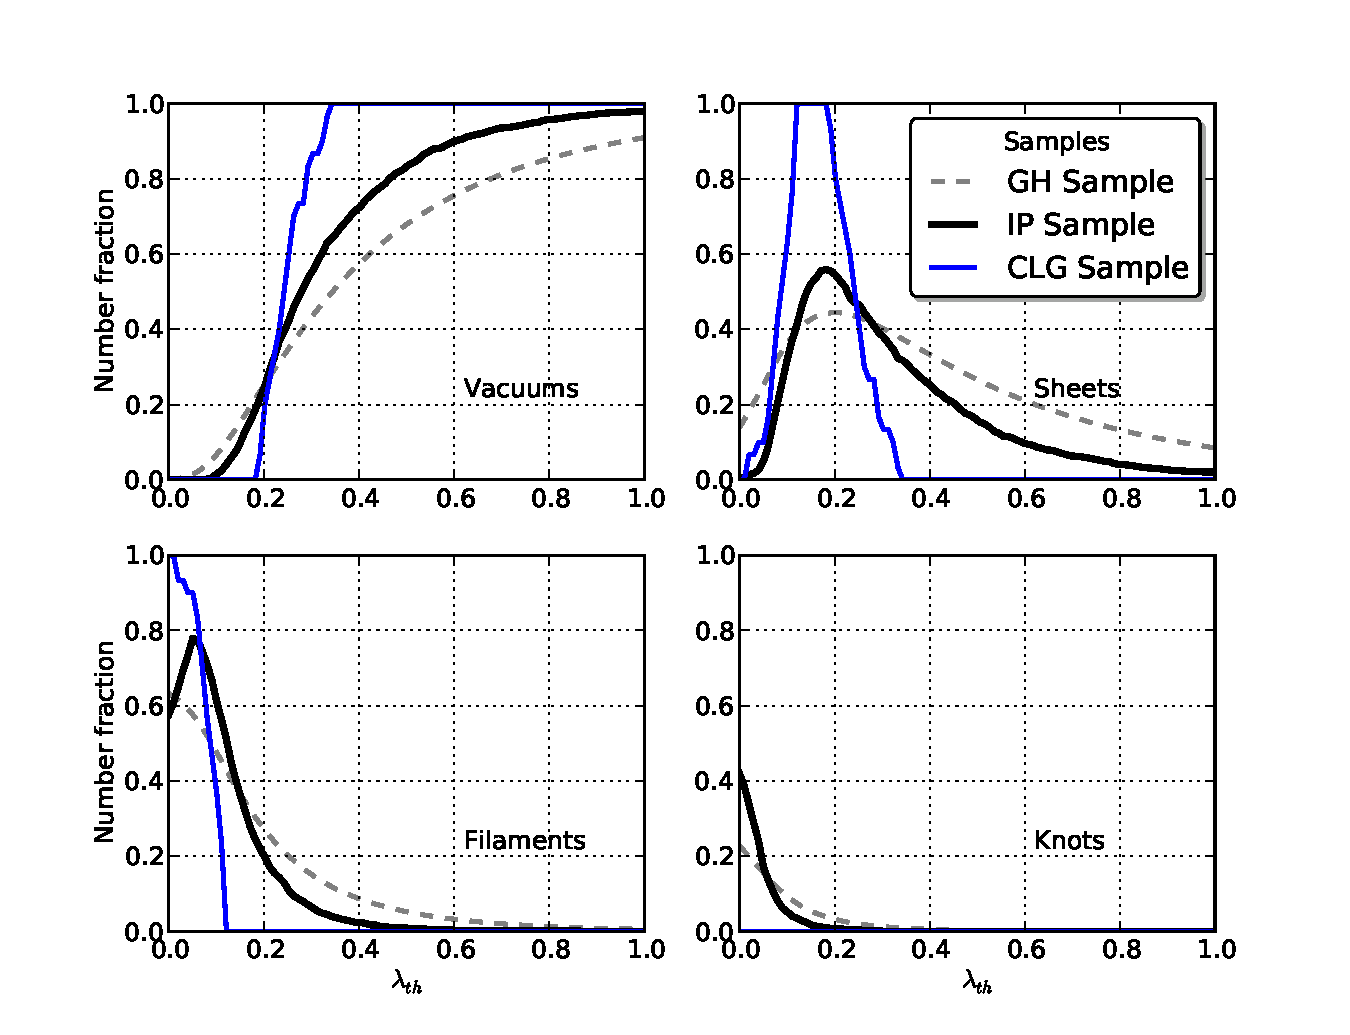
\includegraphics[trim = 8mm 5mm 12mm 12mm, clip, width=0.85\textwidth]
	{./figures/4_results/CLG_Classification_Env.pdf}
	
	\caption{\small{Object fractions in different regions in terms of the
	threshold value $\lambda_{th}$. In the case of the \textit{GH} sample,
	it is counted the number of halos, whereas for the \textit{IP} and 
	\textit{CLG} samples it is counted the number of pair systems.}}
	\label{fig:Samples_Fraction}
\end{figure}
%.........................................................................


%Reviewed
In spite of the classification scheme used, the above conclusions depend
on the selected $\lambda_{th}$ parameter, and although it has been 
reasonably bounded in an optimal region where it is reproduced de visual
impression, it is still a free parameter. In order to solve this, it is 
introduced the fractional of anisotropy (FA) with the normalization used
in \cite{libeskind2013}


%.........................................................................
%Fractional Anisotropy
\eq{eq:FA}
{ FA = \frac{1}{\sqrt{3}}\sqrt{ \frac{ (\lambda_1 - \lambda_3)^2 + 
(\lambda_2 - \lambda_3)^2 + (\lambda_1 - \lambda_2)^2}{ \lambda_1^2 + 
\lambda_2^2 + \lambda_3^2} } }
%.........................................................................


%Reviewed
This quantity allows to quantify the anisotropy degree of the local cosmic
environment, being $FA=1$ a highly anisotropic region, whereas $F=0$ is 
instead a highly isotropic region. Furthermore this quantity is independent
of any free parameter chosen a priori. According to the result obtained by
\cite{libeskind2013}, regions of low isotropy would correspond to knots 
due to their characteristic isotropic collapse, while regions of high 
isotropy would correspond to vacuums due to their non-uniform expansion. 
In the case of filament an sheet regions, the fractional anisotropy is 
extendedly distributed over middle values, thus indicating that the 
dynamic of these type of regions is more complex. Even so, there is a 
slight tendency towards low values in the case of filaments and high 
values for sheets.


%.........................................................................
%Anisotropy Fractional for pairs samples
\begin{figure}[htbp]
	\centering
	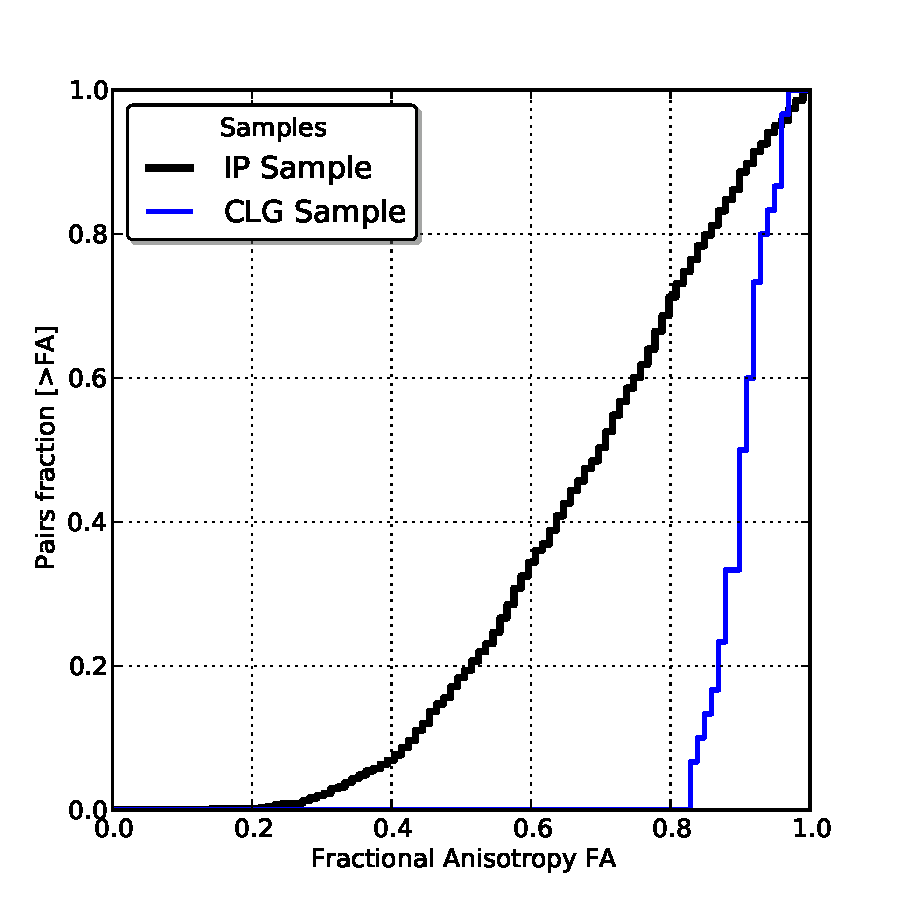
\includegraphics[trim = 0mm 0mm 0mm 10mm, clip, width=0.8\textwidth]
	{./figures/4_results/CLG_FA_Hist.pdf}
	
	\caption{\small{Integrated histogram of the fractional anisotropy for
	the \textit{IP} and \textit{CLG} samples.}}
	\label{fig:FA_samples}
\end{figure}
%.........................................................................	


En la figura \ref{fig:FA_samples} son calculados los histogramas integrados
del fraccional de anisotropía para las muestras \textit{IP} y \textit{CLG}.
El primer resultado está asociado a la distribución de los \textit{IP}, 
la cual es altamente homogénea para rangos intermedios (aproximadamente 
$0.4 < FA < 0.9$) como es evidenciado en la pendiente constante del 
histograma. Esto implica que los sistemas \textit{IP} están distribuidos
en zonas de media a alta anisotropía, en concordancia con las fracciones 
encontradas en regiones de vacío, hojas y filamentos. El segundo resultado
es el sesgo obtenido en la distribución de FA de la muestra \textit{CLG}.
A diferencia de los \textit{IP}, esta distribución se encuentra concentrada 
en regiones de alta anisotropía (aproximadamente $0.8 < FA < 1.0$), lo que
confirma finalmente que es posible asociar un tipo de entorno cosmológico a 
los sistemas \textit{CLG} y el cual esta acorde con regiones vacías y 
planas, o en términos de las direcciones definidas en la V-web, regiones 
que se expanden en dos direcciones (asociadas a los autovalores 
$\lambda_2$ y $\lambda_3$), mientras que poseen un ligero colapso/expansión 
en la tercera dirección (asociada al autovalor $\lambda_1$). 


La principal ventaja de usar el fraccional de anisotropía radica en que 
esta cuantifica en un solo valor la dinámica del entorno cosmológico, 
permitiendo establecer un marco de estudio más natural y directo para 
correlaciones de entorno con cantidades fisicas.


	%---------------------------------------------------------------------
	%Pairs Mass
	\subsection{Masa de los \textit{CLG}}
	\label{subsec:CLG_Mass}
	%---------------------------------------------------------------------
	

Como fue demostrado en la subsección \ref{subsec:Halos_Properties}, la 
distribución de masa de los halos es consistente entre las diferentes
simulaciones, por tanto se espera que todas las muestras, a excepción de 
\textit{CLG} que requiere además del entorno cosmológico, sean también
consistentes entre las simulaciones. Para el estudio de las masas de los
sistemas de pares se propone el uso de dos cantidades, la primera es la
masa total del sistema $M_{tot} = M_A + M_B$ y la segunda es la relación 
de las masas $\chi = M_B/M_A$, donde por convención $M_A$ es el halo más 
masivo.


En la siguiente figura \ref{fig:CLG_Mass} se calculan los histogramas 
integrados para la masa total y la razón de las masas. Se toma la muestra
\textit{IP} como muestra de control, además se muestran los valores 
obtenidos para cada uno de los grupos locales en CLUES.


%.........................................................................
%Integrated Mass Fraction
\begin{figure}[htbp]
	\centering
	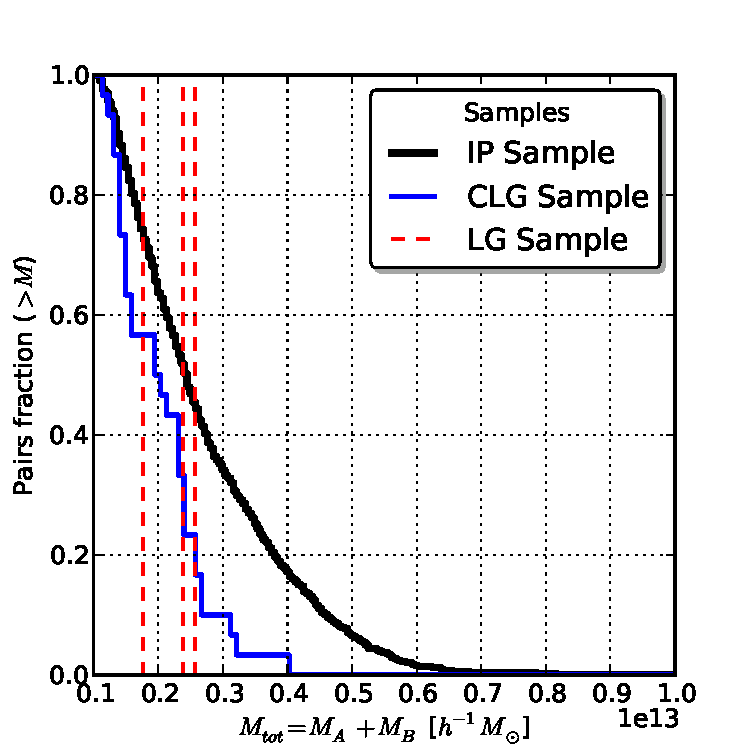
\includegraphics[trim = 0mm 0mm 9.5mm 10mm, clip, width=0.45\textwidth]
	{./figures/4_results/IP_IMF.pdf}
	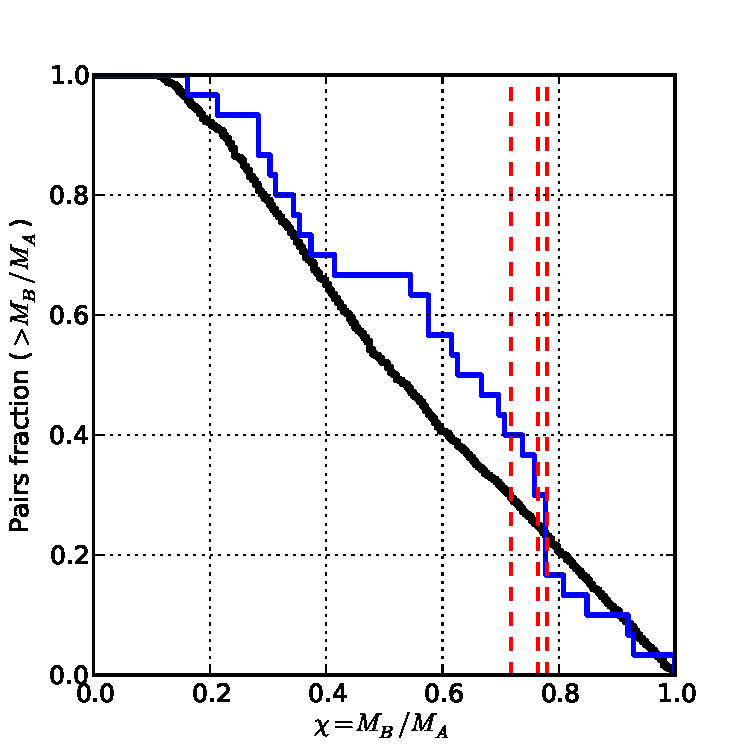
\includegraphics[trim = 0mm 0mm 9.5mm 10mm, clip, width=0.45\textwidth]
	{./figures/4_results/IP_Mass_Ratio.pdf}
	
	\caption{\small{ Funciones de distribución integrada para la masa total
	$M_{A} + M_{B}$ (izquierda) y la razón de las masas $M_B/M_A$ (derecha), 
	de las muestras de pares en Bolshoi. }}
	\label{fig:CLG_Mass}
\end{figure}
%.........................................................................


Una característica interesante de esta figura consiste en los rangos bien 
definidos asociados a la muestra \textit{LG} de CLUES (líneas rojas 
verticales). Esto evidencia que los grupos locales \textit{LG} no solo 
comparten una entorno cosmológico común sino también una distribución de 
masa local. Como posible explicación a esto puede considerase un efecto de 
selección de las muestras en la construcción de las simu\-laciones 
restringidas, mientras que una alternativa optimista sería tomarlo como 
una evidencia de la correlación entre la distribución de masa y el entorno 
local.


Para responder la anterior cuestión se debe analizar la distribución de
los pará\-metros de masa para las demás muestras. En el caso de la masa
total de los \textit{IP}, esta se encuentra distribuida acorde a 
la distribución de masa de los halos (ver figura \ref{fig:IMF}), tal 
como es esperado al no existir ninguna restricción respecto al 
entorno y en el caso de la razón de masas, se obtiene una distribución
completamente homogénea. Ahora, para la muestra \textit{CLG}, la cual se 
espera que sea influenciada por los efectos del entorno, se obtiene una 
distribución de masa total sesgada respecto a la de \textit{IP} y centrada 
aproximadamente en el rango definido por los \textit{LG}. Para la 
distribución de la razón de masas de \textit{CLG} también se encuentra 
un comportamiento uniforme teniendo en cuenta la escasez de datos, 
a pesar de esto hay una aparente sobreabundancia en torno al valor medio 
definido por los \textit{LG}, pero nuevamente no hay suficientes datos 
para concluir una posible relación.

\newpage
%.........................................................................
%Dispersion diagram for pairs mass parameters
\begin{figure}[htbp]
	\centering
	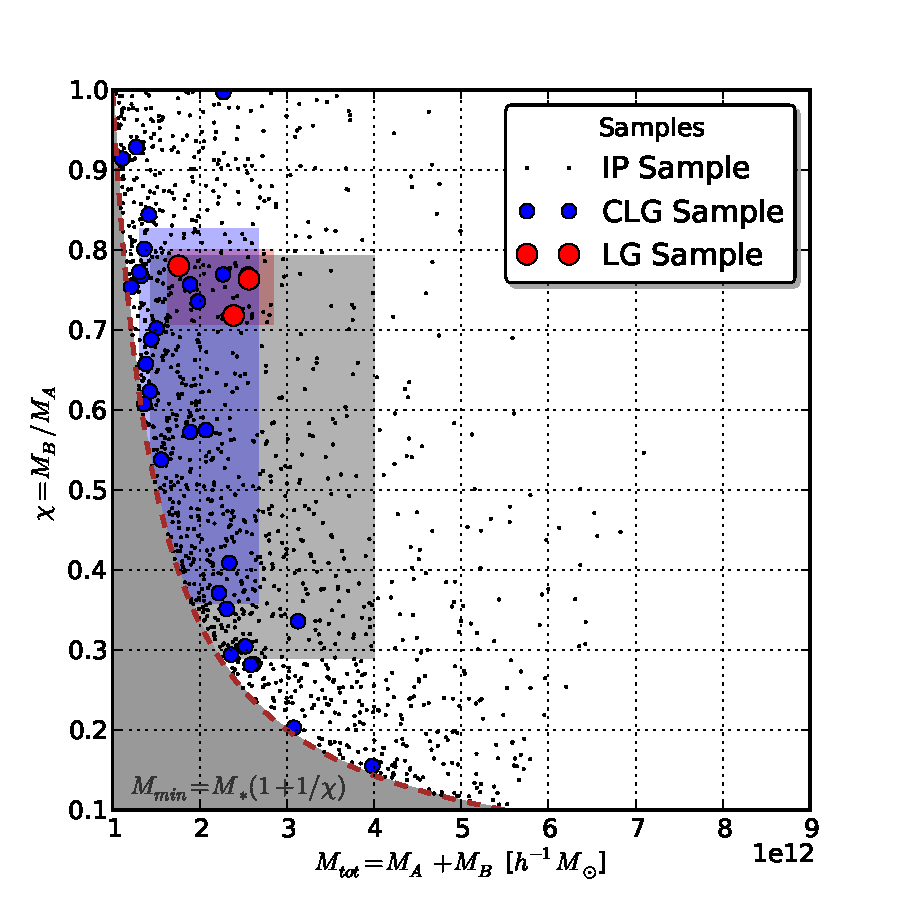
\includegraphics[trim = 0mm 0mm 0mm 10mm, clip, width=0.8\textwidth]
	{./figures/4_results/IP_Mass_vs_Ratio.pdf}
	
	\caption{\small{Diagrama de dispersión de los parámetros de masa 
	definidos ($M_{tot}$,$\chi$) para cada una de las muestras de pares.
	Las regiones cuadradas son construidas a partir del valor medio y la
	desviación estándar de la muestra del mismo color.
	La región gris en la parte inferior izquierda corresponde a un corte
	impuesto artificialmente con el rango mínimo de masa de los halos 
	tomados $M_*$ para construir las muestras de pares.}}
	\label{fig:Dispersion_Mass_CLG}
\end{figure}
%.........................................................................


En la figura \ref{fig:Dispersion_Mass_CLG} se muestra un diagrama de 
dispersión para los parámetros de masa de las muestras de pares. Las 
regiones cuadradas representan el valor medio más o menos una desviación
estándar para las parámetros marcados en cada eje, lo que permite comparar
gráficamente las distribuciones. De esta comparación se confirma que el 
criterio de construcción de la muestra \textit{CLG} selecciona masas de 
pares $M_{tot}$ consistente con las masa de los \textit{LG} en las simulaciones 
restringidas, mientras que no hace ninguna selección respecto a la razón 
de masas $\chi$.


Finalmente, con el objetivo de responder si existe un posible efecto de 
entorno en la selección de la masa total obtenida para la muestra 
\textit{CLG}, se calcula en la siguiente figura \ref{fig:CLG_FA_Mass} 
diagramas de correlación entre el fraccional de anisotropía y los parámetros 
de masa.

\
%.........................................................................
%Correlation Mass-FA
\begin{figure}[htbp]
	\centering
	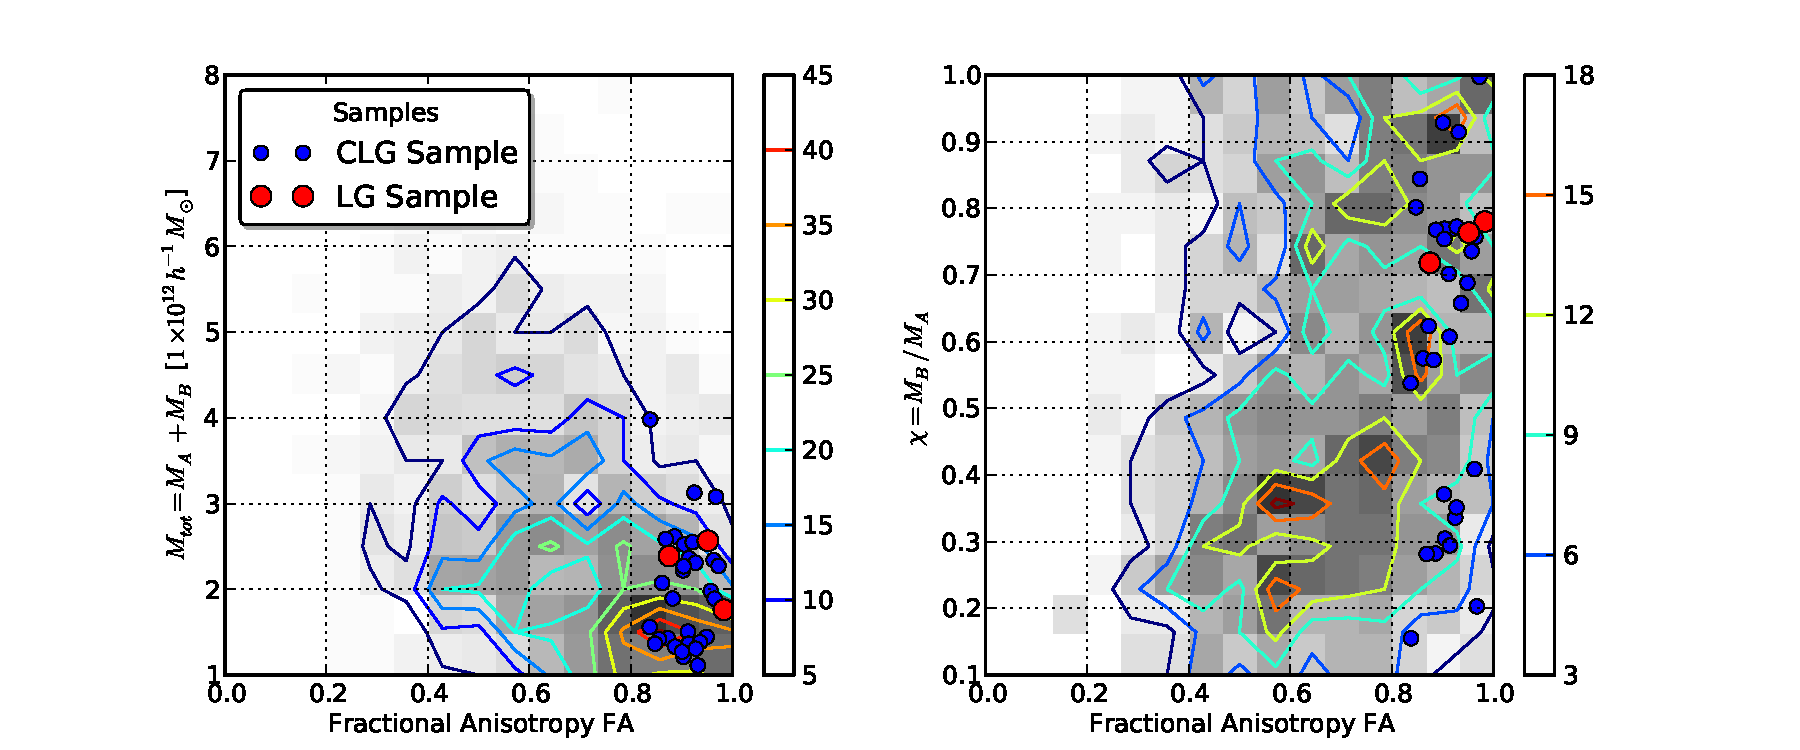
\includegraphics[trim = 25mm 0mm 35mm 10mm, clip, width=1.0\textwidth]
	{./figures/4_results/CLG_FA_Mass.pdf}
	
	\caption{\small{Diagramas de dispersión para el fraccional de 
	anisotropía respecto a los parámetros de masa. El mapa de fondo y las
	curvas de contorno corresponden a número de pares de la muestra 
	\textit{IP}.}}
	\label{fig:CLG_FA_Mass}
\end{figure}
%.........................................................................
\

En el caso de la masa total $M_{tot}$ de la muestra \textit{IP}, puede 
notarse que pares con bajos valores de masa están preferencialmente en 
regiones de alta anisotropía, mientras que pares de masa más alta en 
regiones de anisotropía intermedia. Esto puede ser considerado como una 
correlación de entorno para la muestra \textit{IP} respecto a la masa total, 
de lo cual se concluye que el criterio de selección de la muestra \textit{CLG}
a partir del entorno de los \textit{LG} hace un corte para pares de baja 
masa.


Para la razón de las masas $\chi$ se nota una distribución más dispersa 
para la muestra \textit{IP}, a pesar de esto se nota una sobreabundancia 
de pares con valores de $\chi$ bajos en zonas de anisotropía media, 
mientras que en regiones de alta anisotropía se presentan valores más altos
de $\chi$. Esto es consistente con la selección realizada en la muestra
\textit{CLG}, para la cual aproximadamente el $66\%$ de los pares tienen
un valor $\chi>0.5$. De esto puede intuirse una posible correlación entre
el entorno y el valor $\chi$ de los pares, aún así, debido a la alta 
dispersión de la distribución y la poca cantidad de datos, no puede 
concluirse nada al respecto.
\newpage

	%---------------------------------------------------------------------
	%Angular momentum and energy
	\subsection{Distribuciones de Energía y Momentum Angular}
	\label{subsec:AngularMomentumAndEnergy}
	%---------------------------------------------------------------------


La energía y el momentum angular constituyen otras propiedades físicas de
interés para los sistemas de pares, estas son definidas acá a partir de las
siguiente expresiones


%.........................................................................
%Energy of Pairs
\eq{eq:EnergyPairs}
{ e_{tot} = \frac{1}{M_A + M_B}\cor{ \frac{1}{2}\pr{ M_A v_A'^2 + M_B v_B'^2 } 
 - G\frac{M_A M_B}{| \bds r_A' - \bds r_B' |}}
 }
%.........................................................................


%.........................................................................
%Angular Momentum of Pairs
\eq{eq:AMomentumPairs}
{ \bds L_{orb} = \frac{1}{M_A + M_B}\cor{ M_A\bds r_A' \times \bds v_A' + 
M_B\bds r_B' \times \bds v_B' }}
%.........................................................................
donde $\bds r_i'$ es la posición comóvil del halo $i$ y $\bds v_i'$ es la 
velocidad total\footnote{Velocidad total debido a que se incluye la velocidad 
peculiar y el flujo de Hubble respecto al centro de masa del sistema, así 
$\bds v_i' = \bds v_{pec,i} + H_0 \bds r_i'$. } respecto al centro de 
masa del par.


%.........................................................................
%Energy-AMomentum Dispersion
\begin{figure}[htbp]
	\centering
	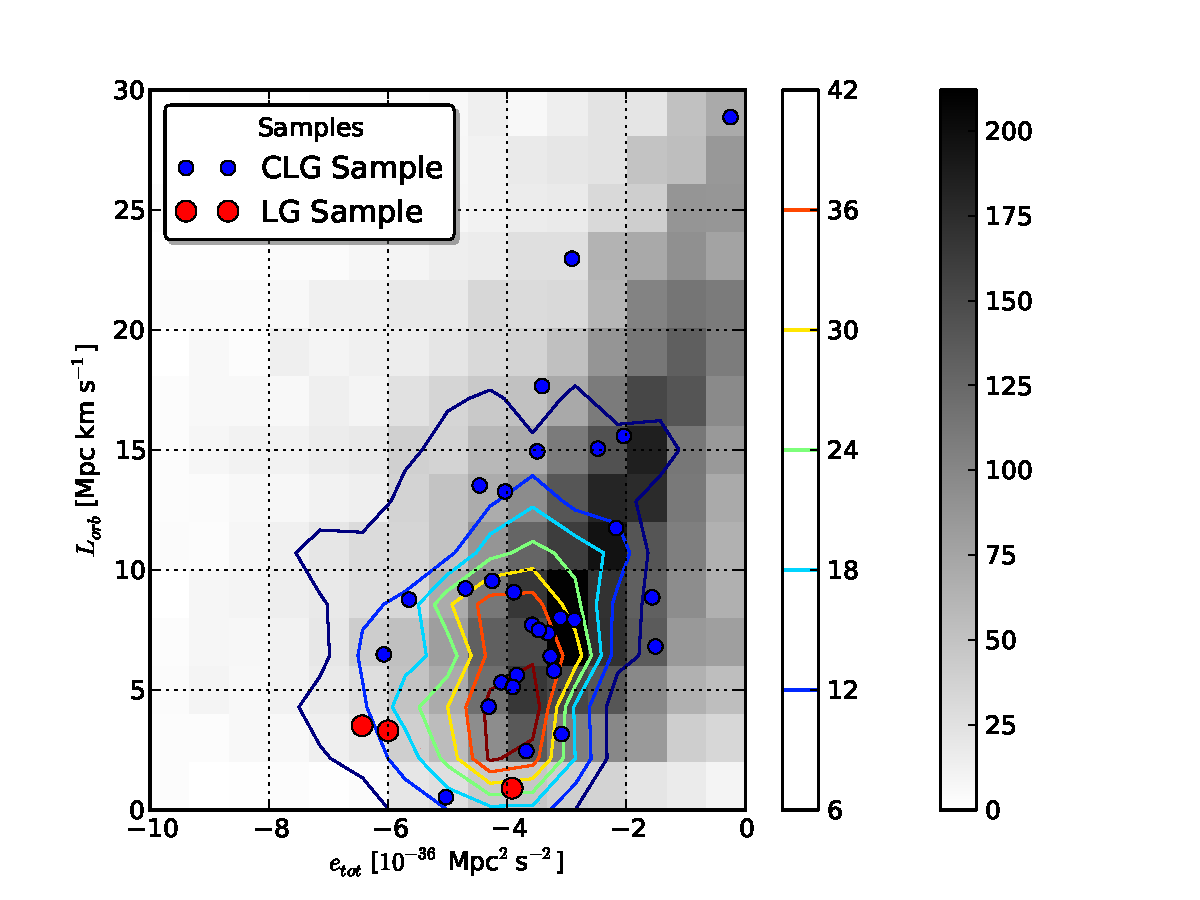
\includegraphics[trim = 8mm 0mm 25mm 10mm, clip, width=0.8\textwidth]
	{./figures/4_results/CLG_E_vs_L.pdf}
	
	\caption{\small{Diagrama de dispersión para la energía total y el 
	momentum angular orbital de los sistemas de pares. El mapa de fondo
	corresponde a la distribución de la muestra \textit{P}, mientas las
	líneas de contorno a la distribución de la muestra \textit{IP}, en 
	ambos casos los valores corresponden al número de pares. }}
	\label{fig:CLG_E-L}
\end{figure}
%.........................................................................	


En la figura \ref{fig:CLG_E-L} se muestran las distribuciones de energía 
total específica y momentum angular orbital específico para las diferentes 
muestras. Lo primero que puede ser notado es un significativo sesgo entre
la distribución de los \textit{IP} respecto a los \textit{P}, lo que 
demuestra que el criterio de aislamiento gravitacional definido en la 
subsección \ref{subsec:SampleOfPairsToUse} selecciona un rango de energía 
y momentum angular más bajo que en los pares generales, siendo así estos 
sistemas gravitacionalmente más ligados. En el caso de la muestra 
\textit{CLG}, su distribución parece seguir la de los \textit{IP},
no habiendo así una aparente selección por la condición entorno. Por último,
es interesante observar nuevamente que las propiedades asociadas a la
muestra \textit{LG} poseen valores muy cercanos, indicando así que
representan un tipo de sistema bien definido, aunque como ha sido mencionado,
esto puede ser efecto de selección en la construcción de CLUES.

\
%.........................................................................
%Correlation Energy, L_orb-FA
\begin{figure}[htbp]
	\centering
	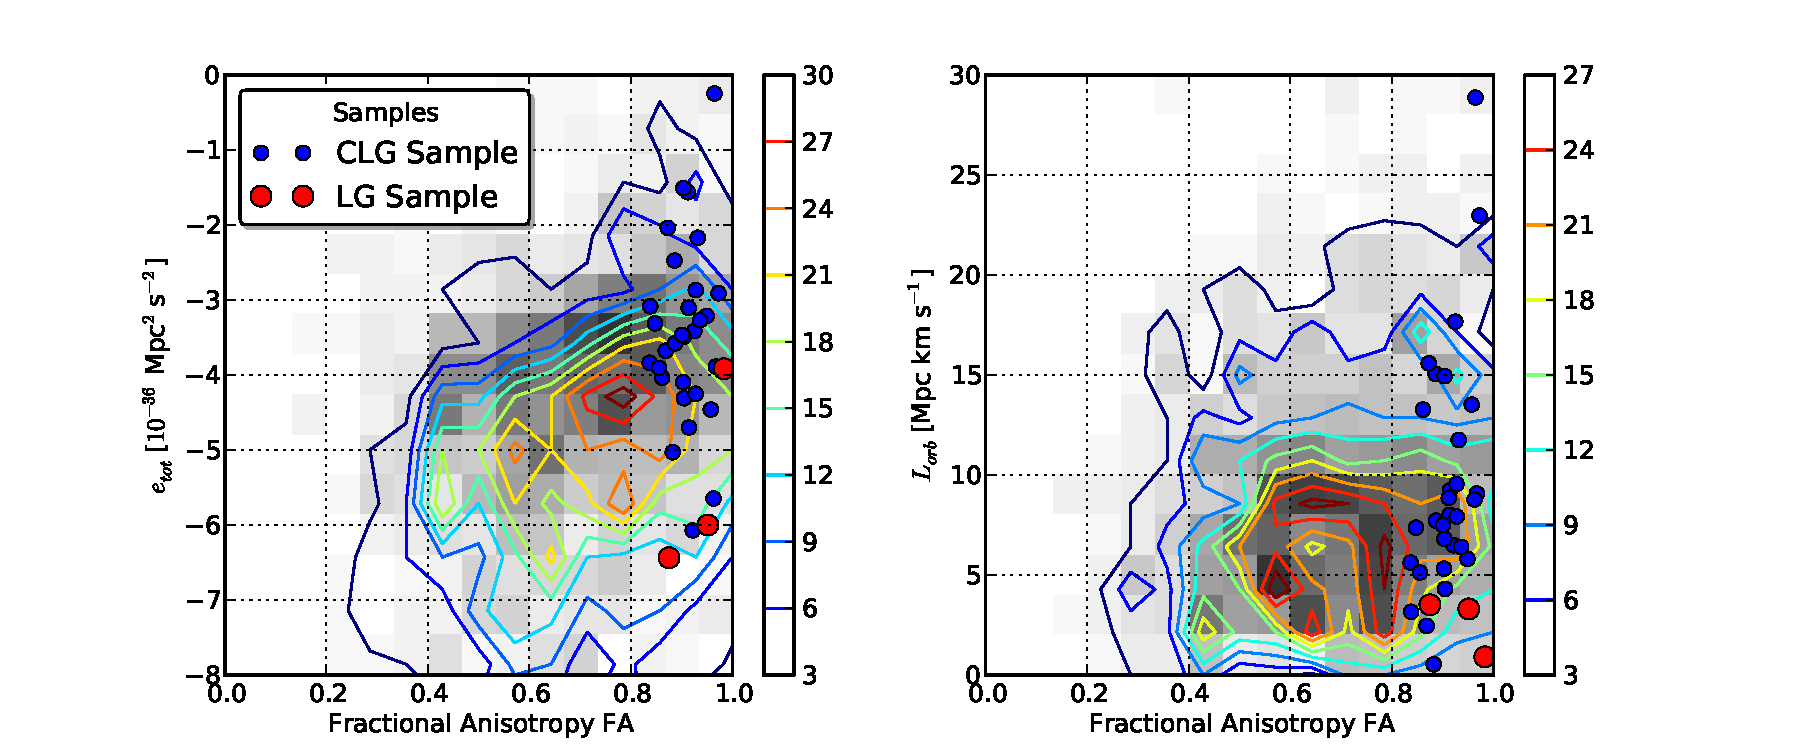
\includegraphics[trim = 20mm 0mm 35mm 10mm, clip, width=1.0\textwidth]
	{./figures/4_results/CLG_FA_E-L.pdf}
	
	\caption{\small{Diagramas de dispersión para el fraccional de 
	anisotropía respecto a la energía y el momentum angular. El mapa de 
	fondo y las curvas de contorno corresponden a número de pares de 
	la muestra 	\textit{IP}.}}
	\label{fig:CLG_FA_E-L}
\end{figure}
%.........................................................................


En la figura \ref{fig:CLG_FA_E-L} se calculan diagramas de correlación de
la energía y el momentum angular con el fraccional de anisotropía con el 
objetivo de determinar posibles correlaciones. En el caso de la energía
específica, sistemas de pares \textit{IP} con mayor energía (menos ligados) 
parecen estar mayoritariamente en zonas de alta anisotropía, mientras que
sistemas de menor energía (más ligados) están en zonas de anisotropía media,
lo que muestra una correlación entre estas dos cantidades. Para sistemas
\textit{CLG}, la selección a partir del entorno parece sesgar su 
distribución de energía a valores más altos que la distribución media de los
\textit{IP}, lo que es consistente con la correlación encontrada. En este
caso, los sistemas \textit{LG} parecen no seguir esta correlación, teniendo
valores mucho más bajos de energía que lo esperado. Finalmente, para la 
distribución de momentum angular específico no existe ninguna correlación 
clara, siendo cualquier valor $L_{orb}$ de los pares igualmente probable 
en el espectro de posibles entornos para estos sistemas.


	
	%---------------------------------------------------------------------
	%Alineación del momentum angular
	\subsection{Alineación del Momentum Angular}
	\label{subsec:AngularMomentumAlineation}
	%---------------------------------------------------------------------
	
	
Finalmente la última propiedad analizada para los sistemas de pares es su
alineación respecto al entorno cosmológico, para esto se define el ángulo
$\phi_i$ como el formado entre el autovector $\bds u_{\lambda i}$ de la
V-web y el momentum angular del par $\bds L_{orb}$.

	
%.........................................................................
%CLG Alineation
\begin{figure}[htbp]
	\centering
	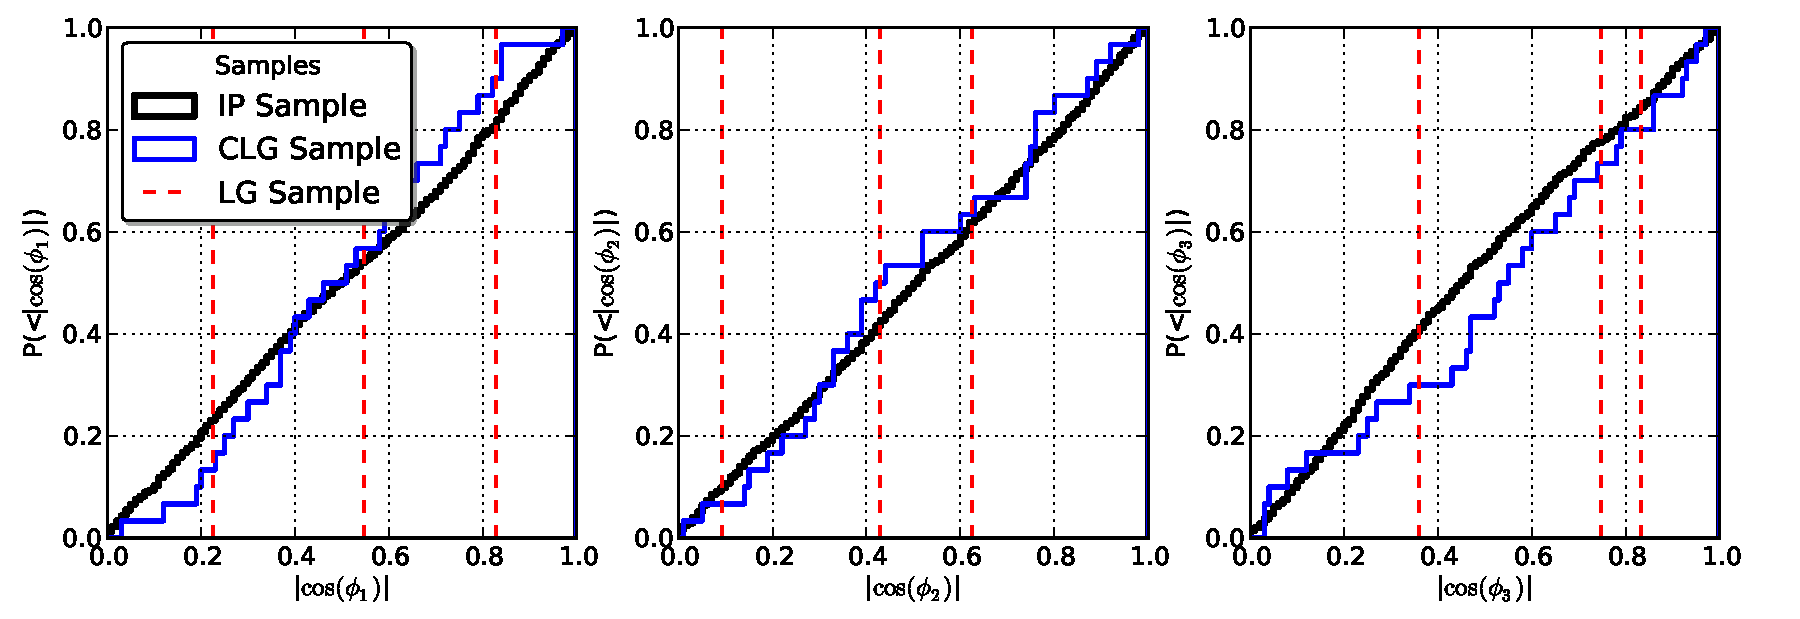
\includegraphics[trim = 0mm 0mm 5mm 0mm, clip, width=1.0\textwidth]
	{./figures/4_results/CLG_Alineation.pdf}
	
	\caption{\small{Histogramas integrados para el ángulo formado entre el 
	momentum angular de los pares, el cual determina el plano orbital, y
	cada uno de los autovectores definidos por la V-web en el entorno
	cosmológico. Se realiza para cada las muestras de pares \textit{CLG} y 
	\textit{IP}, mientras que los grupos locales de CLUES son ilustrados 
	con las líneas rojas punteadas.}}
	\label{fig:CLG_Alineation}
\end{figure}
%.........................................................................
	

En la figura \ref{fig:CLG_Alineation} se calculan los histogramas 
integrados para cada uno de los angulos $\phi_i$ definidos. Como puede 
notarse, las muestras \textit{CLG} y \textit{IP} son homogéneas respecto
a los tres valores, indicando que no hay una alineación preferida respecto
al entorno cosmológico. Esto también se evidencia en los valores calculados
de los \textit{LG} de las simulaciones restringidas.


%*************************************************************************



	
%*************************************************************************
%Conclusions
\section{Conclusiones}
\label{sec:Conclusions}


Esta sección está dedicada a compilar los principales resultados obtenidos
en este capítulo. Estos serán enumerados y discutidos acorde al órden en
que fueron obtenidos.


%.........................................................................
%Main Results
\begin{enumerate}
\item[\textbf{1.}] La construcción de la muestra \textit{IP} fue 
inicialmente propuesta en \cite{forero2011} con el objetivo de reproducir
sistemas tipo grupo local. A pesar de esto, el número de estos sistemas 
encontrados en la simulación Bolshoi es mucho mayor al que se espera acorde
a la abundancia de \textit{LG} en simulaciones restringidas. El método 
propuesto para la selección de la muestra \textit{CLG} en Bolshoi a partir 
del entorno cosmológico de los \textit{LG}, produce un número de sistemas 
que concuerda con los encontrados en la simulaciones restringidas, escalando 
apro\-ximadamente como el volumen de las simulaciones. Más aún, aplicando 
este mismo método en las simulaciones restringidas se halla una muestra
con un tamaño similar a la \textit{LG}.


\item[\textbf{2.}] A partir de los valores medios de densidad en las 
diferentes regiones del entorno cosmológico (figura \ref{fig:Vol_Fraction})
se propone un esquema para la elección de un rango óptimo del parámetro
$\lambda_{th}$ de la V-web con el objetivo de reproducir la 
apariencia visual de la red cósmica. Este está basado en la 
minimización de la densidad media en las regiones de vacío debido a que
son las dominan la apariencia del campo de densidad a gran escala. Con
esto se garantiza que las regiones vacías no invadan regiones de más alta
densidad, que en principio deben ser clasificadas como hojas o filamentos.
Este método da un rango de valores óptimos aproximadamente igual para 
todas las simulaciones usadas ($0.2 \leq \lambda_{th} \leq 0.4$), además
reproduce adecuadamente la apariencia visual (ver figura 
\ref{fig:Vweb_Comparison} para $\lambda_{th} = 0.3$). A pesar de esto, 
este parámetro sigue siendo libre y no es viable usar un esquema de 
clasificación basado en este para determinar correlaciones con propiedades
físicas, en vez de esto se introduce el fraccional de anisotropía 
con la normalización usada en \cite{libeskind2013}.


\item[\textbf{3.}] La distribución del entorno cosmológico de las 
simulaciones Bolshoi y CLUES difieren, existiendo un cambio de densidad 
media muy pronunciado entre regiones de vacío y filamentos en Bolshoi, 
mientras que es mucho más suave en las CLUES. A pesar de esto, las 
fracciones de volumen asociadas a cada tipo de entorno son aproximadamente 
iguales para ambas simulaciones en el rango óptimo determinado para 
$\lambda_{th}$. A pesar de esto, se espera que la dinámica local 
caracterizada por la V-web sea independiente de la estructura global 
de la distribución de entorno, lo cual valida el esquema de selección 
de la muestras \textit{CLG} en Bolshoi.


\item[\textbf{4.}] El método de construcción de los 
\textit{CLG} selecciona un entorno cosmológico común para estos 
sistemas, siendo preferidas zonas de vacío y hojas no muy planas.
Estas regiones presentan una alta anisotropía, cuantificada por el 
fraccional de anisotropía FA. En el caso de los sistemas \textit{IP},
estos se encuentran en zonas de media a alta anisotropía, asociadas 
a valores de baja densidad, contrario a los halos que están en zonas 
más densas y menos anisotrópicas como filamentos y nudos, aún así 
la distribución de entorno de los \textit{IP} es amplia y no pueden
ser asociados a un tipo de entorno específico. El sesgo producido
entre los \textit{IP} y los halos generales se debe al criterio
de aislamiento gravitacional usado para construir los \textit{IP},
esto hace que zonas con mayor densidad de halos sean menos aptas por
la alta influencia gravitacional.


\item[\textbf{5.}] Se encuentra una correlación entre la masa total de 
los pares de la muestra \textit{IP} y el fraccional de anisotropía del 
entorno, donde masas mayores son más abundantes en regiones de 
anisotropía media mientras masas menores se presentan con mayor 
frecuencia en zonas de alta anisotropía. Esto implica que la selección
de entorno realizada en los \textit{CLG} reproduce un rango de masa menor.
En el caso de la razón de masa, no se encuentra ninguna correlación 
significativa con el entorno, aún así se nota una ligera sobreabundancia 
de razones de masa mayores en regiones más anisotrópicas, pero es 
necesaria más estadística para poder ser algo concluyente.


\item[\textbf{6.}] Se halla un correlación para la energía específica
de los sistemas \textit{IP} respecto al entorno, obtiendo valores más
altos en regiones más anisotrópicas y valores bajos en regiones de 
anisotropía media. Esta correlación parece seleccionar un rango de 
energía para los sistemas \textit{CLG}, aunque esta no es consistente
con los valores obtenidos de los \textit{LG}. Para el momentum angular
no se encuentra ninguna correlación con el entorno.


\item[\textbf{7.}] Finalmente se encuentra que no existen alineaciones
privilegiadas entre el momentun angular de los pares \textit{CLG} (o de 
su plano orbital) y las direcciones de los autovectores de la V-web.


\end{enumerate}
%.........................................................................


%*************************************************************************